% !Mode:: "TeX:UTF-8"
%% 请使用 XeLaTeX 编译本文. 适用于 TeX Live 2015 . 本模板的更新下载地址: http://aff.whu.edu.cn/huangzh/
\documentclass{WHUPhd}  % 选项 [forprint]: 交付打印时, 加上此选项, 以消除链接文字之彩色, 避免打印偏淡.
                                      % 选项 [forlib]: 提交给图书馆的电子版, 需要加上选项 forlib, 以消除空白页和彩色链接.
%%%=== 参考文献=== %%%
\bibliographystyle{abbrv}        % 参考文献样式,  plain,unsrt,alpha,abbrv 等等
%%%%%%%%%%%%%%%%%%%%%%%%%%%%%%%%%%%%%%%%%%%%%%%%%%%%
\begin{document}
%%%%%%%-------------------------------------------------

\fenleihao{O159}  % 分类号:《中国图书资料分类法》的类号. 必填. 要根据自己的学科方向填写!!
\miji{}                % 密级
\UDC{}               %《国际十进制分类法UDC》的类号. 选填.
\bianhao{10486}  % 学校编号, 10486是武汉大学的编号. 不用改动.

\title{武汉大学博士论文~\LaTeX~模板}
\Etitle{A \LaTeX~Thesis Template for Wuhan University} % 英文题目
\author{黄正华}
\Eauthor{HUANG Zhenghua}            %作者英文名
\Csupervisor{胡宝清\quad 教授}        %指导教师中文名、职称
\Esupervisor{Prof.~HU Bao Qing}     %指导教师英文名、职称
\Cmajor{数学、计算数学}                   %  学科、专业名称
\Emajor{Computational Mathematics}% 专业英文名
\Cspeciality{智能计算}                     % 研究方向
\Especiality{Intelligent Computing}   % 研究方向
\Schoolname{School of Mathematics and Statistics} %学院英文名. 不确定的话, 请看一下自己学院的网页上是怎么写的. 别搞错了!
\date{二〇一六年五月一日}               %  要注意和英文日期一致!!
\Edate{May 1, 2016}                 % 英文封面日期

%-----------------------------------------------------------------------------
\pdfbookmark[0]{封面}{title}         % 封面页加到 pdf 书签

\maketitle

%-----------------------------------------------------------------------------
% !Mode:: "TeX:UTF-8"

%%% 说明: 此部分需要自己填写的内容:  论文创新点.

%%% ``郑重申明'' 和``论文使用授权协议书'' 分别在 statement.tex 和 protocol.tex 中, 无需改动.

%%%%%%%%%%%%%%%%%%%%%%%%%%%%%
%%% -------------  英文封面 (无需改动)-------------   %%%
%%%%%%%%%%%%%%%%%%%%%%%%%%%%%
\thispagestyle{empty}
\renewcommand{\baselinestretch}{1.5}  %下文的行距
\vspace*{0.5cm}

\begin{center}{\zihao{2} \the\Etitle \par}\end{center}

\vfill

\begin{center}
\zihao{4}
\begin{tabular}{ r l }
 Candidate:      &  {\sc \the\Eauthor}      \\
 Supervisor:     &  {\sc \the\Esupervisor}   \\
 Major:          & \the\Emajor  \\
 Speciality:     & \the\Especiality
\end{tabular}

\vspace*{2cm}
\begin{center}
  \iflib % 向图书馆提交电子文档, 使用黑白校徽.
  
\includegraphics[height=4cm]{whu.eps}       %%  黑白的. 很小, 只有 10k.
  \else
     \ifprint % 文档打印, 使用黑白校徽.
  
\includegraphics[height=4cm]{whu.eps}       %%  黑白的.
  \else
  
\includegraphics[height=4cm]{whulogo.eps} %%  彩色的.
  \fi
  \fi
\end{center}


\zihao{-2}
\the\Schoolname\\
{\sc Wuhan University}

\vspace*{1.0cm}

\the\Edate

\end{center}
%%%%%%%--判断是否需要空白页-----------------------------
  \iflib
  \else
  \newpage
  \thispagestyle{empty}
  \cleardoublepage
  \fi
%%%%%%%-------------------------------------------------
{\pagestyle{empty}
%%%--- 加入``郑重声明'' --- %%%%%%%%%%%%%%%%%
% !Mode:: "TeX:UTF-8"
%%-----------------------论文原创性声明-----------------------------------------%
\newpage
\vspace*{20pt}
\begin{center}{\ziju{0.8}\zihao{-2}\heiti 论文原创性声明}\end{center}
\par\vspace*{30pt}
\renewcommand{\baselinestretch}{2}
{\zihao{4} \songti %



本人郑重声明: 所呈交的学位论文, 是本人在导师指导下, 独立进行研究工作所取得的研究成果.
除文中已经标明引用的内容外, 本论文不包含任何其他个人或集体已发表或撰写的研究成果.
对本文的研究做出贡献的个人和集体, 均已在文中以明确方式标明.
本声明的法律结果由本人承担. 

\vskip2cm

\hspace*{4cm}学位论文作者(签名): \hspace{4cm} \hfill \\[1cm]
\hspace*{10cm}年 \hfill  月 \hfill 日\hspace{1cm}\hfill\par}

%%%%%%%--判断是否需要空白页-----------------------------
  \iflib
  \else
  \newpage
  \cleardoublepage
  \fi
%%%%%%%-------------------------------------------------
\renewcommand{\baselinestretch}{1.6}
\small\normalsize
%%%%%%%%%%%%%%%%%
%%% ---加入``武汉大学学位论文使用授权协议书'' ---  %%%%%%
% !Mode:: "TeX:UTF-8"

%%%%%---武汉大学学位论文使用授权协议书---%%%%%%%%%%%%
%%%%%%%%%%%%%%%%%%%%%%%%%%%%%%%%%%%
%%%%%%%%%%%%%%%%%%%%%%%%%%%%%%%%%%%
\newpage\vspace*{20pt}\thispagestyle{empty}
\begin{center}{\zihao{-2}\heiti 武汉大学学位论文使用授权协议书}\end{center}
\par\vspace*{30pt}

本学位论文作者愿意遵守武汉大学关于保存、使用学位论文的管理办法及规定,
即:学校有权保存学位论文的印刷本和电子版, 并提供文献检索与阅览服务;
学校可以采用影印、缩印、数字化或其它复制手段保存论文;
在以教学与科研服务为目的前提下, 学校可以在校园网内公布部分及全部内容.
\begin{enumerate}[1、]
  \item  在本论文提交当年, 同意在校园网内以及中国高等教育文献保障系统(CALIS)、高校学位论文系统提供查询及前十六页浏览服务.
  \item  在本论文提交~$\Box$~当年/~$\Box$~一年/~$\Box$~两年
            /~$\Box$~三年以后,同意在校园网内允许读者在线浏览并下载全文,学校可以为存在馆际合作关系的兄弟高校用户提供文献传递服务和交换服务.(保密论文解密后遵守此规定)
\end{enumerate}

\vskip 15mm

论文作者(签名):\raisebox{-1ex}{\underline{\makebox[5cm][c]{}}}
\vskip2em
				          				
学\qquad\qquad\quad 号:\raisebox{-1ex}{\underline{\makebox[5cm][c]{}}}
\vskip2em	
					
学\qquad\qquad\quad 院:\raisebox{-1ex}{\underline{\makebox[5cm][c]{}}}					

\vskip  2cm
\begin{flushright}
 日期:\hskip2cm 年\hskip1.2cm 月\hskip1.2cm 日
\end{flushright}

%%%%%%%%%%%%%%%%%%%%%%%%%%%%%%%%%%%%%%%
%%%%%%%--判断是否需要空白页-----------------------------
  \iflib
  \else
  \newpage
  \thispagestyle{empty}
  \cleardoublepage
  \fi
%%%%%%%-------------------------------------------------
%%%%%%%%%%%%%%%%%%
%%%%%%%%%%%%%%%%%%%%%%%%%%%%%%%
}




%%%%%%%%%%%%%%%%%%%%%%%%%%%%%%%
%%% ------------------- 论文创新点----------------------- %%%
%%%%%%%%%%%%%%%%%%%%%%%%%%%%%%%

\newpage\vspace*{20pt}\thispagestyle{empty}
\begin{center}{\zihao{-2}\heiti 论文创新点}\end{center}
\par\vspace*{30pt}
\baselineskip=20pt


  本文的主要创新点在于:

\begin{enumerate}[(1)]
  \item  给出了武汉大学博士毕业论文 \LaTeX{} 模板. 说明了编译方法.

  \item  强调了公式排版的一些细节. 并用例子说明.

  \item  强调了标点符号等的用法. 指出了初学者的一些常见错误.


\end{enumerate}

















%%%%%%%%%%%%%%%%%%%%%%%%%%%%%%%
%%%%%%%--请勿删除以下内容 -------------------------------%
%%%%%%%--判断是否需要空白页-----------------------------%
  \iflib
  \let\cleardoublepage\clearpage
  \else
  \newpage
  \thispagestyle{empty}
  \cleardoublepage
  \fi
%%%%%%%---------------------------------------------------%



    % 加入英文封面, 论文创新点, 等等目录之前的部分.
\frontmatter
\pagenumbering{Roman}               % 正文之前的页码用大写罗马字母编号.
%---把目录加入到书签---%%%%%%%%%%%%%%
\pdfbookmark[0]{目录}{toc}%%%%%%%%%%%%
\pagestyle{oldplain}
\tableofcontents
\pagestyle{oldplain}\cleardoublepage
\newpage  \pagestyle{fancy} \fancyfancy
%------------------------------------------------------------------------------
% !Mode:: "TeX:UTF-8"

%%% 说明: 此部分需要自己填写的内容:  (1) 中文摘要及关键词 (2) 英文摘要及关键词

%%%%%%%%%%%%%%%%%%%%%%%
%%% ------------ 中文摘要 ---------------%%%
%%%%%%%%%%%%%%%%%%%%%%%
\begin{cnabstract}
本文主要介绍和讨论了武汉大学硕士毕业论文的~\LaTeX~模板.
指明了编译方法, 强调了公式排版的一些细节问题, 也指出了一些常见的排版错误.



\end{cnabstract}
\vspace{1em}\par\vfill

%%%--------- 关键词 -------- %%%
\cnkeywords{毕业论文, \LaTeX{}, 模板, XeLaTeX }

%%%%%%%%%%%%%%%%%%%%%%%


%%%%%%%%%%%%%%%%%%%%%%%
%%% ------------ 英文摘要 ---------------%%%
%%%%%%%%%%%%%%%%%%%%%%%

\begin{enabstract}
This thesis is a study on the theory of \dots.




\end{enabstract}
\vspace{1em}\par\vfill

%%%------ 英文关键词 ------- %%%
\enkeywords{\LaTeX{}, XeLaTeX, \dots}


      % 加入中英文摘要.
%------------------------------------------------------------------------------
\mainmatter %% 以下是正文
\baselineskip=20pt  % 正文行距为 20 磅
%%%%%%%%%%%%%%%%%%%%%%%%%%%%%%%%%%%%

\chapter{先说重要的}

本文在 TeX Live 2015 软件环境下, 使用 XeLaTeX 引擎, 可以顺利编译.
TeX Live 的安装方法, 请移步查看: \url{http://aff.whu.edu.cn/huangzh/}.


\section{文档具体使用步骤}

\begin{description}
  \item[Step 1]  进入 includefile 文件夹,  打开 frontmatter.tex,  midmatter.tex,  backmatter.tex 这几个文档,
        分别填写 (1) 论文创新点, (2) 中文摘要、英文摘要, (3) 致谢、发表作品列表.

  \item[Step 2]  打开主文档 PhdTemplate.tex, 填写题目、作者等等信息, 书写正文.

  \item[Step 3]  使用 XeLaTeX{} 编译. 具体见 \ref{sec-compile} 节.

\end{description}


\section{编译的方法}\label{sec-compile}

默认使用 XeLaTeX 编译, 直接生成~pdf 文件.

若另存为新文档, 请确保文档保存类型为 \verb|:UTF-8|. 当然目前很多编辑器默认文字编码为 UTF-8.
WinEdt 9.0 之后的版本都是默认保存为 UTF-8 的.




\section{文档类型选择}
文档类型有 3 种情形:

\begin{table}[ht]\centering
\begin{tabular}{ll}
\hline
   \verb|\documentclass{WHUPhd}|                   &  博士论文 \\
   \verb|\documentclass[forprint]{WHUPhd}|        &  博士论文打印版 \\
   \verb|\documentclass[forlib]{WHUPhd}|           &  博士论文图书馆提交版 \\
\hline
\end{tabular}
\end{table}
相关解释见接下来的两节.


\section{打印的问题}
\begin{enumerate}[i)]
  \item  论文双面打印.
  \item  关于文档选项 forprint: 交付打印时, 建议加上选项 forprint, 以消除彩色链接文字, 避免打印字迹偏淡.
  \item  打印时留意不要缩小页面或居中. 即页面放缩方式应该是``无''(Adobe Reader XI 是选择``实际大小'').
           有可能页面放缩方式默认为``适合可打印区域'', 会导致打印为原页面大小的 $97\%$.
           文字不要居中打印, 是因为考虑到装订, 左侧的空白留得稍多一点(模板已作预留).
  \item  遗留问题: 封面需要打印部重新制作. 比如博士论文要打印书脊, 校内打印部通常有现成的模板.
           我们自己做的封面, 打印部不一定好用.
\end{enumerate}
%如果不是彩色打印机, 请在打印时, 选择将彩色打印为黑白, 否则彩色文字打出的墨迹会偏淡.




\section{提交电子文档}

向武汉大学图书馆提交电子文档, 需单独编译文件: 在文档选项中添加 forlib.

原因: 图书馆要求提交的电子文档不能有空白页、彩色文字.

({\kaishu 这个要求使我在编制模板时遇到了一点问题: 这会导致电子版与纸质版的页码不一致. 博士论文每章的起始页默认在奇数页, 这会不可避免地出现空白页.})


\vfill

本文档下载更新地址: \url{http://aff.whu.edu.cn/huangzh/}. 使用之前, 请移步查看是否有更新.

问题反馈及建议, 请联系: huangzh@whu.edu.cn.

\chapter{杂七杂八的话}

\section{Readme}

模板文件的结构, 如下表所示:
 \begin{table}[ht]\centering
\begin{tabular}{r|r|l}
\hline\hline
  \multicolumn{2}{c|}{PHDTemplate.tex }  &  主文档. 在其中填写正文.\\\hline
  \multicolumn{2}{c|}{WHUPhd.cls} &  定义文档格式的 class file. 不可删除.\\\hline
                          &frontmatter.tex&  英文封面, 论文创新点等. \\\cline{2-3}
 includefile 文件夹  & midmatter.tex  &  中文摘要, 英文摘要等.  \\\cline{2-3}
                            & backmatter.tex &  致谢, 发表作品列表等.  \\\hline
  %\multicolumn{2}{c|}{Adobe fonts 文件夹}  &  Adobe 字体文件, 需自行安装.\\\hline
  \multicolumn{2}{c|}{figures 文件夹} &  存放图片文件.\\\hline
  \multicolumn{2}{c|}{BIBbase 文件夹} &   供 BibTeX{} 做参考文献时选用.\\
\hline\hline
\end{tabular}
\end{table}
%  \footnotetext[1]{定制这个参考文献格式, 主要是希望尽可能满足武汉大学硕士论文的相应格式要求, 比如要求将~article 的``年份''写在``卷号''之前.
%                   存在的问题是: 无法将~book 的``出版时间''标在``出版单位''之前. 事实上, 这个要求有悖于``国家标准~7714-87 文后参考文献著录规则''.
%                   作者名的写法, 依照了``文后参考文献著录规则'', 比如~Albert Einstein 写为~Einstein A.}
%  \footnotetext[1]{编译信息文件常常让我们的文件夹变得凌乱不堪, WinEdt窗口的``垃圾箱''按钮(Erase Output Files),
%     可以让我们方便地删除这些``垃圾''文件. 这也减少了误删文件的可能.}

无需也不要改变、移动上述文档的位置.

可能这里的文档看上去有点多. 如果不习惯用~\verb|\include{ }|~的方式加入``子文档'', 当然可以把它们合并在主文档, 成为一个文档.
({\kaishu 但是这样并不会给我们带来方便.})

%利用~WinEdt~的~Project tree, 可以方便地管理这些文件:
%\begin{itemize}
%    \item 点击~WinEdt~窗口的~Project Tree~按键;
%    \item 再点击~WinEdt~窗口的~Set Main File~按键;
%\end{itemize}
%接下来的管理, 已经清楚地展示在跳出的窗口中了. 再去处理其他的文件时, 还要点击~WinEdt 窗口的~Remove Main File~按键.


英文封面页加了校徽, 有黑白、彩色两种备选, 都是矢量图形, 放大不会失真. 图片文件很小,
用~MetaPost~生成的(准确的说, 是最后一道工序用到了~MetaPost), 过程有点复杂.

本模板首次完成于 2005 年. 历经数次改版. 只记录近期的更新:

%2013 年 12 月更新: 文件夹下放了一个 ntheorem.sty. 是因为有用户遇到了不能编译的问题, 其原因就是需要更新 ntheorem.sty.
%若你知道更新的方法, 感觉这个碍眼, 可以把这个文件去掉. 不知道更新的方法, 就这样放在这里吧.

2014 年 05 月更新: (1) 从中文摘要开始加上页眉. (2) 之前的声明改为``论文原创性声明创'', 内容有改动.
(3) ``学位论文使用授权协议书''内容有改动.

%但是, 研究生院给出的 2014 年的博士论文格式规定, 有多处疏漏和错误, 2015 年应该还有改动.

2015 年 11 月更新: 改造为适应 TeX Live 2015 软件环境.

2016 年 04 月更新: 研究生院公布新的要求. 按此要求修改了封面、论文原创性声明、学位论文使用授权书.

\section{字体调节}

\begin{tabular}{ll}
 \verb|\songti| & {\songti 宋体} \\
 \verb|\heiti| & {\heiti 黑体} \\
 \verb|\fangsong| & {\fangsong 仿宋} \\
 \verb|\kaishu| & {\kaishu 楷书} \\
\end{tabular}


\section{字号调节}
字号命令: \verb|\zihao|

使用 \verb|\zihao| 命令调整字体大小时, 西文字号大小会始终和中文字号保持一致.

\begin{tabular}{ll}
\verb|\zihao{0}| &\zihao{0}  初号字 English \\
\verb|\zihao{-0}|&\zihao{-0} 小初号 English \\
\verb|\zihao{1} |&\zihao{1}  一号字 English \\
\verb|\zihao{-1}|&\zihao{-1} 小一号 English \\
\verb|\zihao{2} |&\zihao{2}  二号字 English \\
\verb|\zihao{-2}|&\zihao{-2} 小二号 English \\
\verb|\zihao{3} |&\zihao{3}  三号字 English \\
\verb|\zihao{-3}|&\zihao{-3} 小三号 English  \\
\verb|\zihao{4} |&\zihao{4}  四号字 English  \\
\verb|\zihao{-4}|&\zihao{-4} 小四号 English \\
\verb|\zihao{5} |&\zihao{5}  五号字 English \\
\verb|\zihao{-5}|&\zihao{-5} 小五号 English \\
\verb|\zihao{6} |&\zihao{6}  六号字 English \\
\verb|\zihao{-6}|&\zihao{-6} 小六号 English \\
\verb|\zihao{7} |&\zihao{7}  七号字 English \\
\verb|\zihao{8} |&\zihao{8}  八号字 English \\
\end{tabular}

按研究生院要求, 本文正文使用的是{\zihao{-4}小四号}.


\section{已加入的常用宏包}

\begin{description}
%  \item[amsmath,amssymb]
  \item[cite]  参考文献引用, 得到形如 [3-7] 的样式.
  \item[color, xcolor]  支持彩色.
  \item[enumerate]  方便自由选择 enumerate 环境的编号方式. 比如

  \verb|\begin{enumerate}[(a)]| 得到形如 (a), (b), (c) 的编号.


  \verb|\begin{enumerate}[i)]| 得到形如 i), ii), iii) 的编号.

\end{description}

另外要说明的是,  itemize, enumerate, description 这三种 list 环境, 已经调节了其间距和缩进,
以符合中文书写的习惯.

\section{标点符号的问题}

建议使用半角的标点符号, 后边再键入一个空格. 特别是在英文书写中要注意此问题!

使用半角也有不足的地方, 比如顿号出不来, 需要临时切换到全角. (当然也有输入法不需要切换, 比如紫光拼音, 可以直接用拼音输入逗号.)

双引号是由两个左单引号、两个右单引号构成的: \verb|``  ''|. 左单引号在键盘上数字~1 的左边.

但是, 无论您偏向于全角或半角, 强烈建议您使用实心的句号, 只要您书写的是自然科学的文章.
原因可能是因为, 比如使用全角句号的句子结尾处的``$x$。''容易误为数学式~$x_0$(\verb|$x_0$|)吧.

\section{中英文间距问题}

使用 XeLaTex 编译将自动加入间距. 不再需要在公式、英文前后加字符``\verb|~|''或空格.

\section{引用的问题}


\subsection{参考文献的引用}

参考文献的引用, 用命令~\verb|\cite{ }|. 大括号内要填入的字串, 是自命名的文献条目名.

比如, 通常我们会说:

 {\kaishu
关于此问题, 请参见文献 \cite{r2}. 作者某某还提到了某某概念\upcite{r1}.}


上文使用的源文件为:

 {\kaishu
关于此问题, 请参见文献~\verb|\cite{r2}|. 作者某某还提到了某某概念~\verb|\upcite{r1}|.
}

其中~\verb|\upcite| 是自定义命令, 使文献引用呈现为\CJKunderdot{上标形式}.

({\heiti 注意:} {\kaishu 这里文献的引用, 有时需要以上标形式出现, 有时需要作为正文文字出现, 为什么?})

另外, 要得到形如~\cite{r1,r3,r4,r5} 的参考文献连续引用, 需要用到 cite 宏包(模板已经加入),
在正文中使用~\verb|\cite{r1,r3,r4,r5}| 的引用形式即可.
或者, 连续引用的上标形式: 使用~\verb|\upcite{r1,r2,r3}|, 得到\upcite{r1,r2,r3}.

\subsection{定理和公式的引用}

\begin{theorem}[谁发现的]\label{th-abcd}
最大的正整数是~$1$.
\end{theorem}

\begin{proof}
要找到这个最大的正整数, 我们设最大的正整数为~$x$, 则~$x \geqslant 1$, 两边同时乘以~$x$, 得到
\begin{equation}\label{eq-abc}
x^2 \geqslant x.
\end{equation}
而~$x$ 是最大的正整数, 由~\eqref{eq-abc} 式得到\footnote{超级链接会出现红色或者绿色的方框, 例如这里的~\eqref{eq-abc}, 这些方框只会在 pdf 电子文档中出现. 打印时, 不会出现该方框.}
\[
x^2 = x.
\]
所以
\begin{equation*}
x = 1.
\end{equation*}
\end{proof}

定理~\ref{th-abcd} 是一个重大的发现.

%%%%----- 定义等环境的举例 --------
\begin{definition}[整数]
 正整数(例如 1, 2, 3)、负整数(例如 ${−1}$, $−2$, $−3$)与零(0)合起来统称为{\heiti 整数}.
\end{definition}

\begin{remark}
  整数集合在数学上通常表示为 $\mathbf{Z}$ 或 $\mathbb{Z}$, 该记号源于德语单词 Zahlen(意为`` 数'')的首字母.
\end{remark}

\begin{proposition}
任意两个整数相加、相减、相乘的结果, 仍然是整数.
\end{proposition}

\begin{example}
  $1+2=3$.
\end{example}

\begin{corollary}
   在整数集合内, 相加、相减、相乘运算是封闭的.
\end{corollary}

\section{图形与表格}

支持 eps, pdf, jpg 等常见图形格式.

再次澄清一个误会: \LaTeX{} 支持的图形格式绝非 eps 这一种. 无需特意把图片转化为 eps 格式.

用形如 \verb|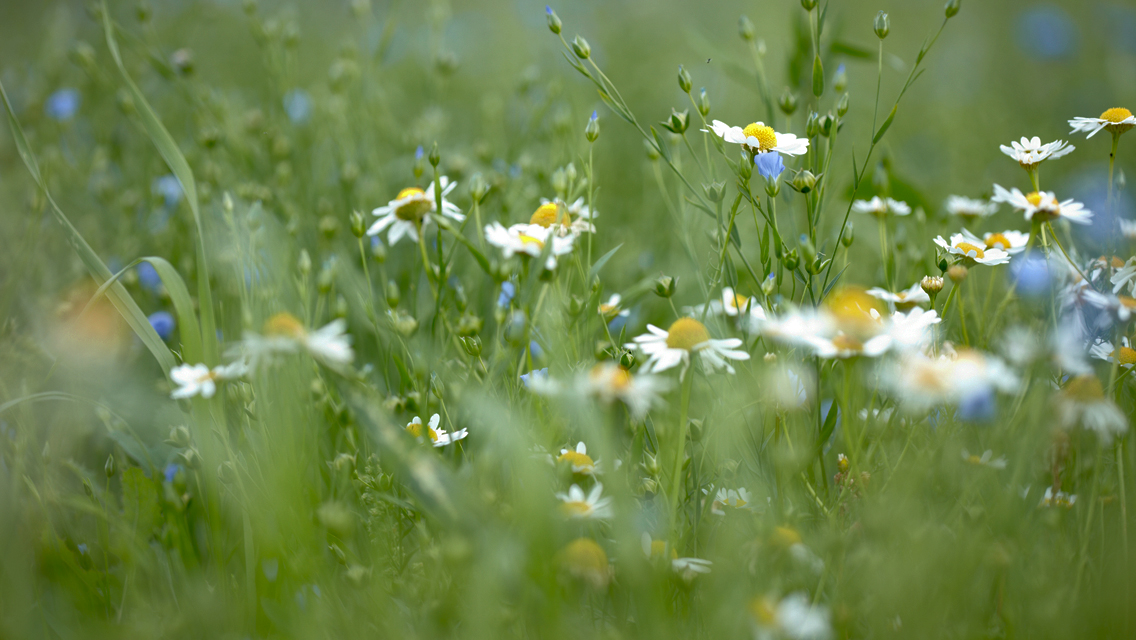
\includegraphics[width=12cm]{Daisy.jpg}| 的命令可以纳入图片.

如图 \ref{fig:1} 是一个纳入~jpg 图片的例子.

\begin{figure}[ht]
\centering
  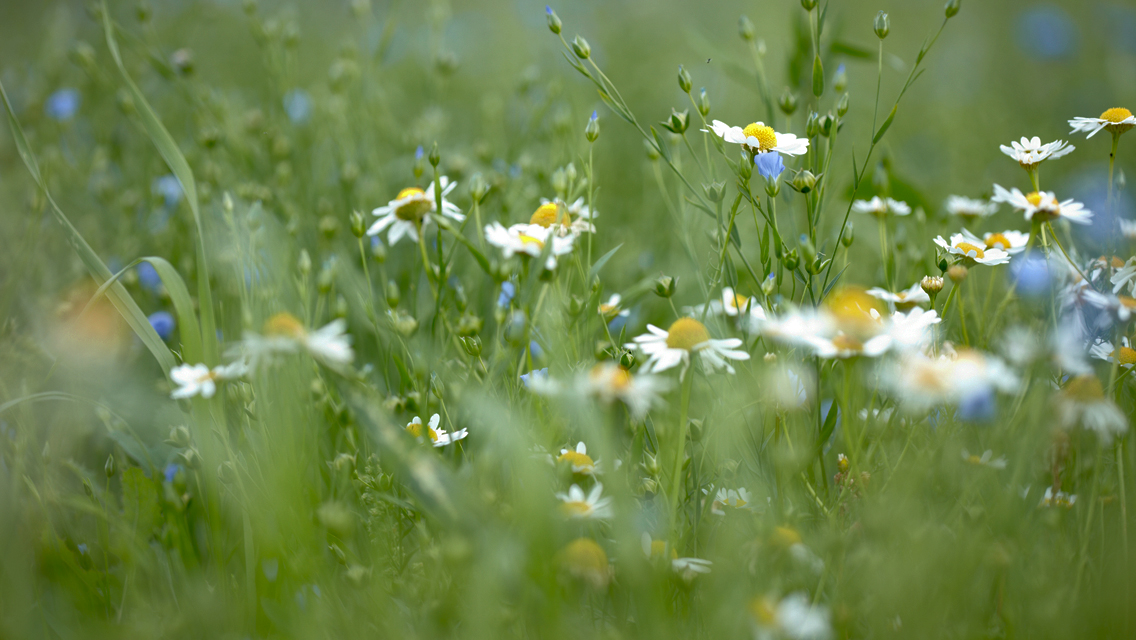
\includegraphics[width=\textwidth]{Daisy.jpg}
  \caption{一个彩色 jpg 图片的例子}
  \label{fig:1}
\end{figure}

表格问题, 建议使用``三线表'', 如表 \ref{tab:1}.

\begin{table}[ht]
\centering
\caption{一般三线表}
\label{tab:1}
    \begin{tabular}{c c c c c c c c c c c}
    \hline
    123 & 4  & 5  & 123 & 4 & 5123 & 4 & 5 & 123 & 4 & 5\\
    \hline
    67 & 890 & 13 & 123 & 4 & 5123 & 4 & 5 & 123 & 4 & 5\\
    67 & 890 & 13 & 123 & 4 & 5123 & 4 & 5 & 123 & 4 & 5\\
    67 & 890 & 13 & 123 & 4 & 5123 & 4 & 5 & 123 & 4 & 5\\
    \hline
    \end{tabular}
\end{table}

%\begin{table}[h]
%  \centering
%  \caption{调整线宽的三线表}\label{tab:2}
%    \begin{tabular}{c c c c c c c c c c c}
%    \hlinewd{0pt}
%    姓名: &&&&年龄: &&&& 性别:\\
%    \hlinewd{1.5pt}
%    123 & 4  & 5  & 123 & 4 & 5123 & 4 & 5 & 123 & 4 & 5\\
%    \hlinewd{1pt}
%    67 & 890 & 13 & 123 & 4 & 5123 & 4 & 5 & 123 & 4 & 5\\
%    67 & 890 & 13 & 123 & 4 & 5123 & 4 & 5 & 123 & 4 & 5\\
%    67 & 890 & 13 & 123 & 4 & 5123 & 4 & 5 & 123 & 4 & 5\\
%    \hlinewd{1.5pt}
%    \end{tabular}
%\end{table}



%%%%==========================================================%%%




\chapter{其他事项}
以下是广告时间, 插播一段广告:
\begin{itemize}
    \item 插图的制作, 建议 TiKz/pgf.
          TiKz/pgf 的长处是源文件直接植入~\TeX~文档, 管理起来非常方便.
    这里有我写的一个关于初次使用~TiKz/pgf~的帖子:\\    \url{http://bbs.ctex.org/forum.php?mod=viewthread&tid=30480}.
    \item 生成参考文献, 建议使用~BibTeX.  这里有我写的一个文档: \\
    \url{http://bbs.ctex.org/forum.php?mod=viewthread&tid=26056}.

      {\kaishu 使用 BibTeX{} 做参考文献时,
      借助 EndNote 或者 NoteExpress, 可以非常漂亮简单地解决 bib 文件的录入问题.
      NoteExpress 在武汉大学图书馆网站有正版软件提供下载.
      当然 EndNote 本身就是 Thomson Corporation 推出的(和 SCI 搜索引擎是同一家公司),
      和多个重要文献搜索引擎有良好的功能配合.

      Google 学术搜索也提供了文献的 bib 格式.
      录入参考文献时, 偶尔用一用 Google 学术搜索, 还可以核查或减少录入的错误, 并减少录入的工作量.}
     \item 幻灯片的制作, 建议使用~Beamer. 这里有我写的一个模板, 谨供参考:\\
    \url{http://bbs.ctex.org/forum.php?mod=viewthread&tid=27695}.

\end{itemize}

%%%=====================================================================%%%
\chapter{武汉大学2016年博士学位论文撰写及印制规格的规定}


{ {\heiti 说明}: \kaishu
 这些规定偶有变动.
 请仔细查阅当年拿到的《武汉大学申请博士学位有关规定》那个红色小本子.
 若发现不一致的地方, 请您发邮件给我: huangzh@whu.edu.cn.}

\bigskip


[原文地址: \url{http://www.gs.whu.edu.cn/index.php/index-view-aid-7956.html}.]
\bigskip

国务院学位办文件规定:研究生学位论文撰写和编印必须符合国家标准局统一编制格式,
并将博士学位论文提交北京图书馆和北京科技信息研究所收入国家级图书编目,
以便及时向社会提供查阅,促进国内外学术交流. 根据文件精神结合我校学位论文归档的要求,
对我校博士学位论文印制规格作出如下规定:

{\heiti 一、论文装订格式的排列顺序}

(一)封面(格式和要求见附页一)

(二)论文英文题目(专用一页纸,上方为题目用宋体2号字,下方为研究生姓名宋体4号字、外文专业应有中文题目)

(三)郑重声明(格式和要求见附页二)

(四)学位论文使用授权书(格式和要求见附页三)

(五)博士生自认为的论文创新点

(六)目录(格式和要求见附页四)

(七)中文摘要

(八)英文摘要

(九)引言

(十)正文(格式和要求见附页五)

(十一)中外文参考文献(格式和要求见附页六)

(十二)攻博期间发表的与学位论文相关的科研成果目录(格式参见附页六:参考文献排列格式)

(十三)后记/致谢

{\heiti 二、论文印制规格及要求}

(一)论文用A4张(210×297mm)标准大小的白纸打印;\colorbox{yellow}{正文部分双面印制}.

(二)论文在打印时,纸张四周留足空白边缘,每页上方(天头)和左侧(订口)应分别留边25mm以上,
下方(地脚)和右侧(切口)分别留边25mm以上.

{\heiti 三、论文封面格式}

(一)分类号. 必须在封面左上角注明分类号,一般应注明《中国图书资料分类法》的类号,
同时尽可能注明《国际十进分类法UDC》的类号.

(二)密级. 论文必须按国家规定的保密条例在右上角注明密级(如系公开型论文则可不注明密级).

(三)编号. 武汉大学编号为10486,标注在封面右上角.

(四)论文题目. 题目必须用楷体标准一号字标注于明显的位置,应是集中概括论文最重要的内容,
一般不超过20个字,以有助于选定关键词和编制题录. 题目不能用缩略词,首字母缩写字、字符、
代号和公式等,题目语意未尽,可用副标题补充说明. 外语专业的论文题目一般采用英文,英文题目不宜超过10个实词.

(五)论文作者姓名.

(六)论文指导教师姓名. 指导教师姓名必须是填写当年被学校批准招收博士生的教师.

(七)专业名称. 专业名称必须是我校已有学位授予权的学科专业,并按国家颁布的学科专业目录中一级学科或二级学科名称印制.

(八)书脊(专指博士学位论文). 书脊上应用仿宋体四号字于上方标明论文题目,下方注明研究生姓名.

(九)论文封面统一用120克铜版纸,封面底色为白色.

(十)论文封面格式要求详见附三页.

{\heiti 四、论文英文题目}

论文英文题目专用一页纸,``英文题目''用宋体二号字,其下``研究生姓名''用宋体四号字;外语专业应为中文题目.

{\heiti 五、郑重声明}


``郑重声明''用黑体小二号字,内容用宋体四号字.

为了加强学风、学术道德建设,规范学术行为,提高学位论文质量,确保学位授予的权威性、严肃性,学校对学位论文撰写特别强调以下几点:

(一)凡申请学位人员须对自己的学位论文负责,在提交的学位论文的英文题目后页(中文摘要前页)增设一页书面声明,即``郑重声明''.

(二)学位论文中的引证、引述处须注明出处.

(三)学位论文后所附参考文献,必须是申请学位人员真正阅读和参考过的文献.

(四)合作科研及成果,应在致谢或后记中有相关说明,避免产权纠纷.

(五)学位论文中没有郑重声明的,不能参加论文答辩.

{\heiti 六、中文摘要}

``中文摘要''用黑体小二号字,内容用宋体小四号字,页码用罗马数字单独编排,并标注在每页页脚中部.

{\heiti 七、英文摘要}

``英文摘要''用加粗Times New Roman小二号字,内容用Times New Roman小四号字,页码续接中文摘要的页码.

{\heiti 八、论文关键词}

每篇论文必须选取3--5个以上中、英文关键词,排在其论文摘要的左下方,用黑体小四号字.

{\heiti 九、目录}

目录是论文的提纲,也是论文组成部分的小标题.
排列顺序是:1、中文摘要 2、英文摘要 3、引言 4、正文章节 5、中外文参考文献 6、攻博期间发表的科研成果目录
7、后记(可不要此项). 并对每项标明页码.

{\heiti 十、引言(绪论)}

论文的页码由引言(绪论)的首页开始,作为第1页,并为右页,一律用阿拉伯数字连续编排页码,必须统一标注在每页页脚中部.

{\heiti 十一、正文}

正文是学位论文的核心部分,必须由另页开始,一级标题之间换页,二级标题之间空行;内容一律用宋体小四号字,
字间距设置为标准字间距,行间距设置为最小值20磅,各章、节应有序号.

{\heiti 十二、参考文献}

参考文献用黑体四号字,内容用宋体五号字.

{\heiti 十三、学位论文印刷份数}

由培养单位根据需要决定印刷份数. 在学位论文定稿后,可先印刷数份给论文评阅人和答辩委员,
然后根据论文评阅人和答辩委员对论文的意见进行修改后,才能正式印刷,提交学校存档.

{\heiti 十四、论文制作时须加页眉}


页眉从中文摘要开始至论文末, 偶数页码内容为``武汉大学博士学位论文'', 奇数页码内容为学位论文题目.


%%=========================================================================%%%
\chapter{论文提交给图书馆}

{\kaishu 以下文字参看武汉大学图书馆网页:
 \begin{center}
 \url{http://www.lib.whu.edu.cn/web/index.asp?obj_id=457&menu=h}.
 \end{center}
 提交论文之前, 请到该网址查看要求是否有新变化.
}

    经研究生院与图书馆共同商议决定, 武汉大学研究生在学位论文答辩通过后,
    采用以下方式提交学位论文:首先进行电子版论文网上提交, 经图书馆审核通过后, 进行纸本论文提交.

\section*{前期准备}
\begin{itemize}
  \item[一、] 请下载《武汉大学学位论文使用授权协议书》(一式两份), 一份论文作者保存, 一份留学校存档.
    留学校存档的协议书事先用钢笔或中性笔填写后,  装订在提交给学校图书馆的纸本论文末页.\footnote{\heiti 特别说明:
    本文前面所附的《武汉大学学位论文使用授权协议书》, 图书馆要求放在最后;
    而研究生院是要求发在文档前面(在论文原创性声明之后). }

    \item[二、]涉密论文缴送到武汉大学档案馆, 由档案馆加盖公章后到图书馆办理相关离校手续.

    \item[三、]电子版论文要求
\begin{enumerate}[1.]
  \item 论文的电子文本应采用 Word 或 PDF 格式编辑(不加密).
  \item 电子版全文包括的内容及顺序应与纸本一致: 包括中英文封面、郑重声明、中英文摘要、目录、引言、正文(含图表)、参考文献及附录, 并放在一个文档中.
  \item \colorbox{yellow}{电子版文档中不能有空白页、标记、彩色字、乱码.}
  \item 目录的页码一定要与正文的章节以及附后的内容相符合. 论文正文页码须从第一页起, 正文之前部分(不包括封面)用罗马字母(I, II, \dots)编页.
\end{enumerate}
\end{itemize}



\section*{电子版论文提交}

    进入图书馆主页(\url{http://www.lib.whu.edu.cn})点击``博硕士论文提交'', 进入论文提交系统.
    具体步骤和注意事项请参见论文提交过程演示(PPT).
    论文提交成功的 3 个工作日后, 可查收 Email 或在``已通过论文名单查询''中查询论文是否审核通过.
    如果提交的论文不合格, 请按邮件要求修改后再次进入系统提交论文.


\section*{纸本论文提交}

    电子版论文提交审核通过的, 请提交 1 份纸本论文到相应的论文纸本缴送地,
    末页须装订一份填写好的协议书.

%%%------------附录. 不需要的话, 可以删除.--------
\appendix

\chapter{测试1}

测试

\chapter{测试2}

测试

\chapter{测试3}

测试


%%%=== 参考文献 ========%%%
\cleardoublepage\phantomsection
\addcontentsline{toc}{chapter}{参考文献}
\begin{thebibliography}{000}\zihao{5}

  \bibitem{r1} 刘海洋, 《\LaTeX{} 入门》, 电子工业出版社, 2013.

  \bibitem{r2} ctex.org, 《\CTeX{} 宏集手册》, V2.2, 2015/07/01, \url{http://www.ctan.org/pkg/ctex}.

  \bibitem{r3} 邓建松, 《\LaTeXe~用户手册》.
             \url{http://math.ecnu.edu.cn/~latex/docs/LaTeX2e_manual.zip}.

  \bibitem{r4} Karl Berry 编写, 江疆~翻译, 《\TeX{} Live 指南\ —\ 2015》.
              \url{http://tug.org/texlive/}.

  \bibitem{r5} Herbert Vo\ss, 《Mathmode》, V2.47, 2014, \url{http://www.ctan.org/pkg/voss-mathmode}.

\end{thebibliography}




\backmatter

% !Mode:: "TeX:UTF-8"

%%% 说明: 此部分需要自己填写的内容:  (1) 攻博(硕)期间科研成果 (2) 致谢

%%%%%%%%%%%%%%%%%%%%%%%
%%%------- 攻博(硕)期间科研成果 -------%%%
%%%%%%%%%%%%%%%%%%%%%%%
\reseachresult

\begin{enumerate}[{[1]}]
\item   作者, 文章题目, 期刊名, 年份(期数): 起止页码

\item   作者, 书名, 版次, 出版地:出版单位, 年份, 起止页码
\end{enumerate}


%%%%%%%%%%%%%%%%%%%%%%%
%%% --------------- 致谢 ------------- - %%%
%%%%%%%%%%%%%%%%%%%%%%%
\acknowledgement



感谢你, 感谢他和她, 感谢大家.














%%%%%%%%%%%%%%%%%%%%%%%%%%%%%%%%%%%%%%%
%%%%%%%--判断是否需要空白页-----------------------------
  \iflib
  \else
  \newpage
  %\thispagestyle{empty}
  \cleardoublepage
  \fi
%%%%%%%-------------------------------------------------

 %%%致谢、作品列表 .

\cleardoublepage
\end{document}



